%! Author = R2D2 Team 3
%! Date = 14/04/2020

% Preamble
\documentclass[11pt]{article}
\usepackage{hyperref}
\usepackage{natbib}
\usepackage[official]{eurosym}

\usepackage{graphicx}
\usepackage{tabularx}
\graphicspath{ {./Images/} }

\usepackage{array}

\usepackage{natbib}

\usepackage{xcolor}

\usepackage{color}
\usepackage{colortbl}

\bibliographystyle{apalike}
\renewcommand{\refname}{\section{Referenties}}

\renewcommand{\contentsname}{Inhoudsopgave}

\newenvironment{definition}
    {
        \renewcommand{\arraystretch}{1.2}
        \begin{tabular}{>{\bfseries}l >{\em}p{0.7\textwidth}}
    }
    {
        \end{tabular}
        \renewcommand{\arraystretch}{1}
    }

\newcolumntype{Y}{>{\centering\arraybackslash}X}

\newcommand{\todo}[1]{\textcolor{red}{\emph{#1}}}


\title{Gebruik van Photoplethysmography om hartslag en zuurstofsaturatie te meten in rampgebieden}

\author{\emph{R2D2 Team 3} \and Finn Fonteijn \and Youri de Vor}

% Document
\begin{document}

    \begin{titlepage}
        \centering
        \maketitle
        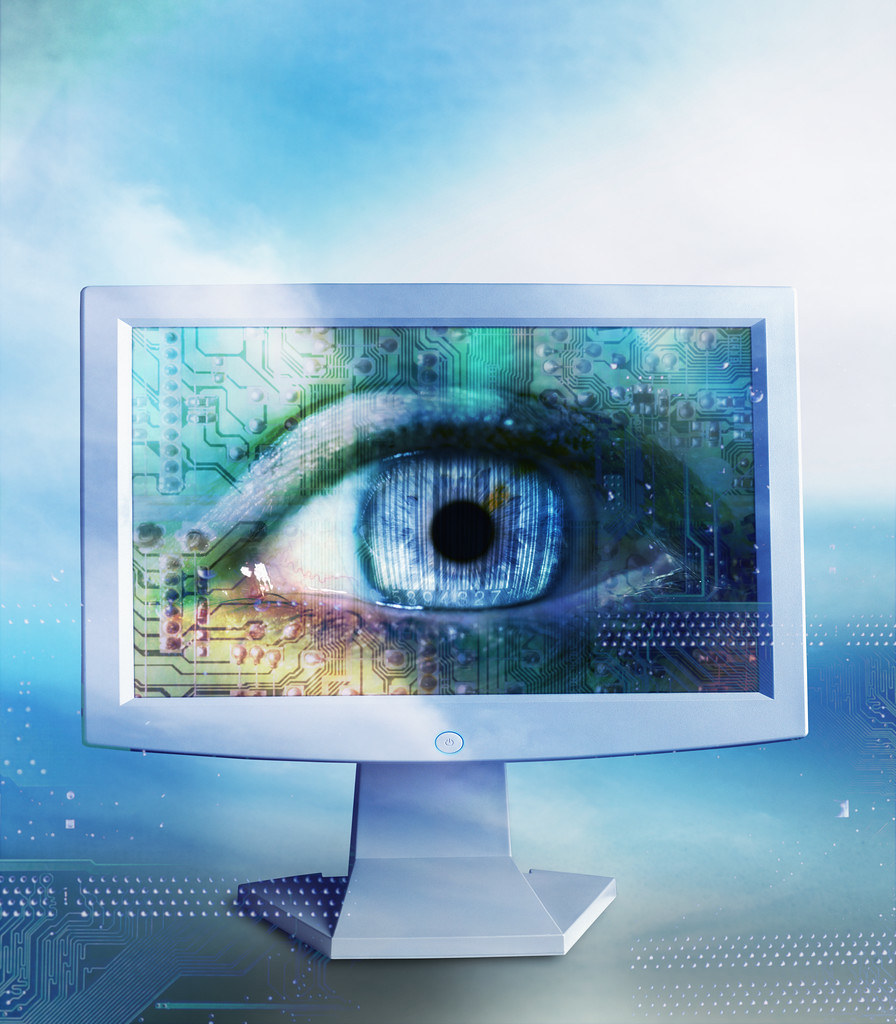
\includegraphics[height=0.6\textheight]{Images/vision.jpg}
        \clearpage
    \end{titlepage}


    \clearpage
    \tableofcontents

    \clearpage

    \section{Abstract}\label{sec:abstract}
    In deze paper doen we literatuuronderzoek naar verschillende methodes voor pijn herkenning en pogen deze te implementeren.
    De methodes die overwogen worden zijn een optical flow aanpak en een methode gebaseerd op het tracken van facial features.

    \section{Voorwoord}\label{sec:voorwoord}
    Dit onderzoek wordt uitgevoerd in opdracht van de Hogeschool Utrecht, voor het project R2D2 2020.
    Bij dit project wordt er een ICT-bedrijf gesimuleerd.
    De werkgroep waaronder dit onderzoek valt is Team 3:\\
    \\

    \emph{
    \begin{tabularx}{\textwidth}{YYY}
        Niels Post & Otto de Visser & Amrit Malhi\\
        Menno van der Jagt & Youri de Vor & Finn Fonteijn\\
        Vincent van Setten & Oscar Kromhout
    \end{tabularx}
    \vspace{1em}
    }

    \section{Inleiding}\label{sec:inleiding}

    Het gebruik van een pulse oximeter geeft je belangrijke informatie over een aantal vitale functies van een slachtoffer. 
    Afhankelijk van de gekozen manier om deze meting uit te voeren, kan dit op een snelle, goedkope en niet-invasieve manier.
    In dit onderzoek kijken we naar verschillende meetmethoden en of deze geschikt zijn voor onze applicatie, letters B en C van de ABCDE methode voor eerste hulp. 
    Letters B en C staan voor breathing en circulation. 
    Vervolgens zullen wij kijken naar de verschillende sensoren die op de markt beschikbaar zijn, en de meest geschikte kiezen voor ons project.


    \section{Probleemstelling}\label{sec:probleemstelling}
    Voor doktoren is het lastig om een objectief pijn vast te stellen.
    Vaak moet een pati\"{e}nt zelfeen getal tussen de 1 en de 10 geven voor zijn pijn.
    Echter is deze manier van pijn inschatten niet erg objectief, daarnaast is het niet
    altijd mogelijk met de pati\"{e}nt te communiceren.
    In rampscenario's zijn er bijvoorbeeld te veel slachtoffers om aan iedereen te vragen hoeveel pijn hij voelt.
    Wel is het belangrijk om te weten hoeveel pijn mensen hebben om ze met meer/minder prioriteit te helpen.
    Hierom, in combinatie met de doelen van het R2D2 bedrijf, bestaat de vraag naar een automatische module die pijn
    detecteert.

    \section{Begrippenlijst}\label{sec:begrippenlijst}
    \paragraph{Triage}
    Triage is een middel om met beperkte capaciteit spoedzorg te organiseren. 
    In de kern betekent triage dat in een tijdsbestek van enkele minuten op basis van beperkte gegevens een beslissing genomen moet worden over hoe snel de patiënt dient te worden beoordeeld door een hulpverlener, zoals een huisarts, ambulanceverpleegkundige of een SEH-arts.    
    bron https://de-nts.nl/nts/basisprincipes-nts/

    \paragraph{PPG} 
    Photoplethysmography (PPG) is een simpele en goedkope optische meetmethode die vaak wordt gebruikt voor het controleren van hartslag doelen. 
    PPG is een niet-invasieve technologie die een lichtbron en een fotodetector op het huidoppervlak gebruikt om de volumetrische variaties in de bloedcirculatie te meten. 
    bron (https://www.ncbi.nlm.nih.gov/pmc/articles/PMC6426305/) Techniek die we gebruiken voor het meten van hartslag/zuurstof saturatie


    \paragraph{SpO2}
    Zuurstofsaturatie Perifeer,  het percentage zuurstofrijk hemoglobine (hemoglobine dat zuurstof bevat) in vergelijking met de totale hoeveelheid hemoglobine in het bloed (zuurstofrijk en niet-zuurstofrijk hemoglobine). 
    Gemeten met een externe sensor op de huid.

    \paragraph{SaO2} 
    Zuurstofsaturatie Slagaderlijk, dezelfde meeting als SpO2 maar dan verkregen via een Bloedgasmeting 


    \section{Literatuurverkenning}\label{sec:literatuur}
    \paragraph{The Feasibility of Using a Forehead Reflectance Pulse Oximeter for Automated Remote Triage(Wendelken 2004)}Het uiteindelijke doel van The Feasibility of Using a Forehead Reflectance Pulse Oximeter for Automated Remote Triage(Wendelken 2004), namelijk Remote Triage, staat heel dichtbij het doel van ons overkoepelende onderzoek. 
    Wedelken et al. kijken of het gebruik van een Reflectance Pulse Oximeter in staat is om nauwkeurig metingen van O2 Sats en Hartslag, zelfs bij signaal ruis veroorzaakt door fysieke inspanning van de proefpersoon.

    \paragraph{Mendelson 2006} heeft een portable pulse oximeter systeem ontworpen voor gebruik in Remote Triage situaties. 
    Het doel van van het systeem komt weer overeen met ons eigen onderzoek. 
    Dankzij de vooruitgangen op technologisch gebied is het ontwerp van het systeem wat verouderd, maar de uitdagingen en methodes kunnen wij nog steeds in acht nemen voor ons eigen ontwerp.

    \paragraph{Heart rate measurement based on time-lapse image} is een interessant onderzoek om te bekijken voor het bepalen van de research gap. 
    Hartslag metingen op basis van een camera zijn relevant omdat het automatisch plaatsen van sensoren voor een robot niet triviaal is. 
    In dit onderzoek is gebruik gemaakt van een toentertijd gangbare handheld camera. 
    Het type sensor van de camera is tegenwoordig niet goed meer te verkrijgen. 
    Dit heeft echter geen invloed op de relevantie van het onderzoek sinds de camera slechts werd gebruikt voor het opnemen van een time lapse. 
    De camera wordt gebruikt om een 30 seconde durende timelapse op te nemen met een interval van 200ms. 
    Het gezicht van de patiënt wordt in deze timelapse vorm opgenomen. 
    Hierna wordt voor een vakje van 3 bij 4 centimeter de gemiddelde intensiteit bepaald en hieruit wordt, na verwerking, een hartslagfrequentie uit gehaald.

    \paragraph{The non-contact monitoring of heart and respiratory rates using laser irradiation: an experimental simultaneous monitoring with and without clothes during biochemical hazards} is zeer relevant vanwege het op afstand meten van hartslag. 
    Dit wordt in dit onderzoek gesimuleerd d.m.v. konijnen. Kleding wordt gesimuleerd door middel van een klein stukje stof op de huid. 
    De metingen van deze methode zijn geverifieerd d.m.v. een ECG.

    \paragraph{Heart rate monitoring system using finger tip through Arduino and Processing Software} is een paper die gaat over het meten van hartslag op de Arduino met PPG. 
    Dit paper beschrijft zo goed als de gewenste methode van meten. 
    PPG sensoren voor de Arduino zijn een kosten effectieve en verkrijgbare hartslagmeter. 
    In de paper wordt de sensor uit losse componenten opgebouwd en wordt er gebruikt gemaakt van een Processing library.


    \section{Theorie en hypothese}\label{sec:theorie-en-hypothese}
    \subsection{Saturatie}
    Een te lage zuurstofsaturatie in het bloed(hypoxemie) kan leiden tot een tekort aan zuurstof toevoer aan organen of weefsel (hypoxie).
    Na enige tijd veroorzaakt dit cel dood[10], tenzij er weer zuurstof beschikbaar komt voor deze getroffen gebieden van het lichaam.

    Lage Zuurstofsaturatie in het bloed kan veroorzaakt worden door een aantal oorzaken [9], in dit onderzoek richten wij ons op oorzaken die zich voordoen na trauma of onderkoeling.
    Acute respiratory distress syndrome(ARDS) komt vaak voor na trauma of longontsteking, en is behandelbaar door reddingswerkers met zuurstof en ventilatie[8]. 
    ARDS en andere problemen met ademen/gaswisselingen in de longen zijn vaak te herkennen aan een te lage zuurstofsaturatie.

    Slagaderlijk Zuurstofsaturatie (SaO2) kan het beste gemeten worden door een Bloedgasmeting. 
    Hierbij wordt een kleine hoeveelheid bloed van een patiënt naar een klinisch-chemisch laboratorium gestuurd en wordt het bloed geanalyseerd en de meting teruggegeven. 
    [goede bron vinden] Hoewel deze methode de meest nauwkeurige resultaten terug geeft, is dit onpraktisch om een een noodsituatie  te moeten doen, en kost het kostbare tijd als een patiënt in ademnood is.

    Echter bestaat er een verband tussen en slagaderlijke zuurstofsaturatie(SaO2) en perifere zuurstofsaturatie(SpO2)[7]. 
    Dit laatste kan gemakkelijk gemeten worden door een sensor aan de buitenkant van de huid(niet invasief). 
    Er zijn bepaalde chronische /bijzondere omstandigheden waar het verschil tussen SpO2 en SaO2 van belang zijn, maar het meten van de perifere zuurstofsaturatie goed genoeg voor patiënten op de Intensive Care.[11] 
    Hierdoor zal in de rest van dit document zuurstofsaturatie altijd wijzen naar de perifere en niet de slagaderlijke zuurstofsaturatie.

    Het meten van de SpO2 wordt gedaan door middel van Photoplethysmography(PPG) Hiervoor wordt een sensor gebruikt die twee LEDs bevat, en een fotodetector. 
    Het Licht van de ene LED heeft een golflengte van 660 nm (Rood) en de andere 940 nm (InfraRood). Deze twee LEDs sturen het licht door een vinger of oor, met de fotodetector aan de weerszijde. 
    De LEDs pulseren dit omstebeurt (met pauzes er tussen om te compenseren voor omgevingslicht) ongeveer 30 keer per seconden. 
    Het geabsorbeerde licht bij deze golflengten verschilt aanzienlijk tussen bloed dat is geladen met zuurstof en bloed zonder zuurstof. 
    Zuurstofrijk hemoglobine absorbeert meer infrarood licht en laat meer rood licht door. Zuurstofarm hemoglobine laat meer infrarood licht door en absorbeert meer rood licht. 
    Vervolgens kan een microcontroller in de sensor gebruik maken van de Beer-Lambert wet om de zuurstofsaturatie uit te rekenen[12]

    Het hierboven beschreven PPG is een zogenoemde transmissive PPG, hierbij wordt het door het medium uitgezonden licht gedetecteerd door een de photodetector tegenover de LED-bron. 
    Het alternatief is een Reflective PPG, hierbij wordt het licht gedetecteerd dat terug gereflecteerd wordt door weefsel, botten en bloedvaten.

    
    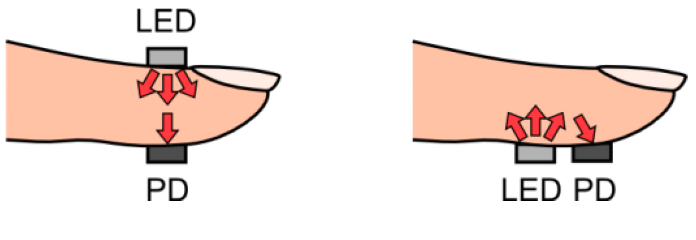
\includegraphics[height=0.2\textheight]{Images/Tamura1.png}

    \citet{tekano2007heart}

    Een transmissive PPG kan een relatief goed signaal verkrijgen, maar de meetlocatie is beperkt. 
    Om een meting te doen moet de sensor zich op het lichaam bevinden op een plaats waar doorgelaten licht gemakkelijk kan worden gedetecteerd, zoals de vingertop, het neustussenschot, de wang, de tong of de oorlel. 
    Het plaatsen van de sensor op het neustussenschot, de wang of de tong is alleen effectief onder anesthesie. 
    De vingertop en de oorlel zijn de voorkeursposities; deze plaatsen hebben echter een beperkte bloedperfusie. 
    Bovendien zijn de vingertop en de oorlel gevoeliger voor extreme omstandigheden, zoals lage omgevingstemperaturen.

    Een Reflective PPG elimineert de problemen die verband houden met de plaatsing van de sensor en er kunnen verschillende meetlocaties worden gebruikt (zoals besproken in de volgende sectie). 
    Reflective PPG wordt echter beïnvloed door bewegingsartefacten en druk storingen. 

    \subsection{Hartslag}
    Op eenzelfde manier kan de hartslag worden gemeten. 
    Volgens [Heart rate monitoring system using finger tip through Arduino and Processing Software] zetten de haarvaten in de huid van een vinger op als gevolg van een stijging in de bloeddruk tijdens een hartslag. 
    Deze verandering in formaat kan worden gemeten d.m.v. PPG.

    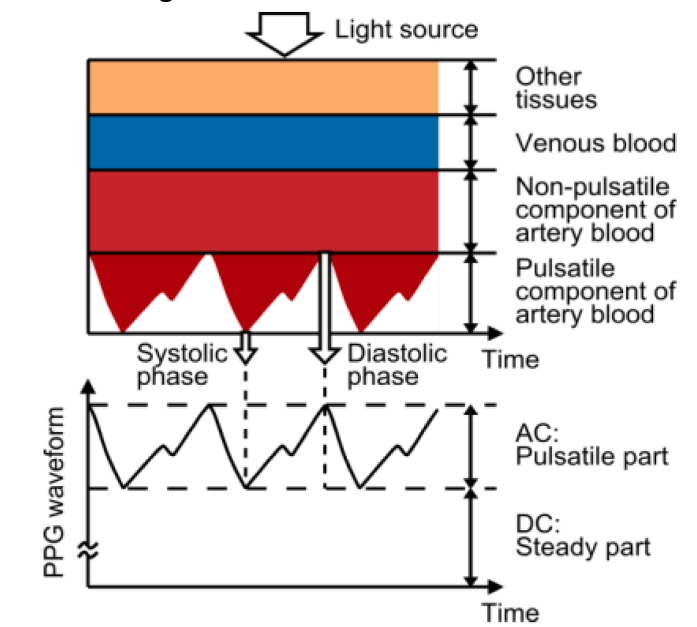
\includegraphics[height=0.5\textheight]{Images/Tamura2.png}

    
    Hartslag is een minstens zo belangrijke metriek als zuurstofsaturatie. Het is algemeen bekend dat zowel een te lage, te hoge als een onregelmatige hartslag kunnen negatieve gevolgen hebben voor de gezondheid. 
    Ook kan er op deze manier vastgesteld worden of de patiënt überhaupt een hartslag heeft.
    Daarnaast is het vaststellen van een hartaanval ook mogelijk door het meten van de onderlinge tussenposes. 

    Te hoge hartslag kan een indicatie zijn van onder andere bloedverlies, koorts, infectie, gebrek. 
    Deze oorzaken zijn veelvoorkomend tijdens rampsituaties aangezien lichamelijke letsel een veel voorkomend gevolg is van een rampsituatie. 
    De gevolgen van een te hoge hartslag zijn kortademigheid, duizeligheid, flauwvallen, zwakte en moeheid.
    [Symptoom Snelle regelmatige hartslag (tachycardie) - Symptomenchecker]

    Te lage hartslag is ook een belangrijke metriek. 
    Dit kan onder andere dienen als indicatie van onderkoeling, bloedingen en een verhoogde hersendruk, naast andere oorzaken. 
    Een te lage hartslag kan leiden tot duizeligheid, kortademigheid, vermoeidheid, hartkloppingen, flauwvallen, en geheugenstoornissen. 
    [Bradycardie (te lage hartslag) - hoe herken je het?]

    misschien nog iets over pleth waves als we dit verder gebruiken.



    \section{Uitvoering}\label{sec:uitvoering}
    \subsection{Deelvraag 1 tot en met deelvraag 4}\label{subsec:deelvraag-1-tot-en-met-deelvraag-4}
    Voor deze deelvragen zullen wij een literatuuronderzoek
    verrichten naar methoden van pijndetectie door middel van Vision.
    Hierbij zullen wij per methode de deelvragen beantwoorden, om zo uiteindelijk een conclusie te kunnen trekken over
    de meest geschikte methode(n).
    Voor het aangeven van de hardware-vereisten maken wij een beredenering waarom wij denken dat er een bepaalde hardware-vereiste is.
    In deze beredenering kijken we vooral naar het geheugengebruik van de methode,
    aangezien dit de meest limiterende factor is van een embedded systeem.

    Om de onderzochte methoden inzichtelijk te maken voor onszelf, beantwoorden wij voor onszelf een aantal vragen over elke methode.
    Omdat de antwoorden op deze vragen niet direct relateren aan de deelvragen, maar een methode inzichtelijk dienen te maken, kan de lezer de antwoorden hierop vinden inde bijlagen.
    Deze vragen zijn als volgt:
    \begin{itemize}
        \item Korte Omschrijving
        \item Van welk principe maakt het gebruik
        \item Geschatte piek-geheugengebruik per meting
        \item Geschatte tijdsduur voor een conclusie
        \item Mogelijkheid om te draaien op een embedded systeem
    \end{itemize}


    Voor \emph{\hyperref[itm:dv1]{deelvraag 5}} doen wij een vergelijkend onderzoek voor camera's.
    We onderzoeken het bestaan van camera's specifiek voor vision, en noteren specificaties van deze camera's.
    Bij dit onderzoek betrekken wij ook een webcam en een actiecamera.

    Voor deelvraag 6 doen wij experimenteel onderzoek.
    Door meerdere implementaties te vergelijken, kunnen wij de maximale bereikbare waarden ervan vergelijken.


    \section{Resultaten}\label{sec:resultaten}

    \subsection{Deelvraag 1 t/m 4}\label{subsec:deelvraag-1-t/m-4}
    \emph{Is het mogelijk om computer vision toe te passen op videobeeld om pijn te kunnen herkennen op het gezicht van een mens?}

    Wij hebben een aantal velden opgesteld die wij per methode hebben onderzocht.
    De volgende resultaten zijn hieruit gekomen

    \subsection{Onderzoek methoden pain detection}\label{subsec:onderzoek-methoden-pain-detection}

    \subsubsection{Methode 1}

    \emph{\citet{werner2014automatic}} Automatic pain recognition from video and biomedical signals\\
    \emph{\citet{prkachin1992consistency}} The consistency of facial expressions of pain: a comparison across modalities\\
    Deze methode combineert het gebruik van Vision algoritmen, met het meten van biomedische data door middel van sensoren.
    Wij zullen hier alleen kijken naar het gedeelte van de methode met betrekking tot Vision.

    \paragraph{Aantal foto's per tijdseenheid}
    Deze methode maakt gebruik van veranderingen in gezichtsafstanden ten opzichte van een baseline, en kan dus met 2 foto's een resultaat geven.
    Deze foto's hoeven dan ook niet extreem snel verwerkt te worden, en het systeem mag hier een aantal seconden over doen.

    \paragraph{Hardware-vereisten}
    De vereisten voor de berekening zelf zijn weinig: Er moeten slechts een aantal afstanden van coordinaten vergeleken worden.
    Dit zullen de meeste microcontrollers ook kunnen.
    Het probleem zit hierom meer in de methode van facial feature detection.
    Afhankelijk van de gebruikte methode, moet de processor mogelijk meerdere kleurafbeeldingen opslaan, en bij convolutie van een afbeelding moet een afbeelding vaak twee keer aanwezig zijn in het geheugen.
    
    \emph{Bij de onderstaande redenering gaan wij uit van onze ervaring in algemene gezichtsdetectie, aangezien wij geen diepgaande ervaring hebben met gezichtseigenschappen-detectie.
    Mogelijk is zo een algoritme dus meer/minder geheugenintensief dan wij aannemen}

    Bij het opslaan van een kleine kleurafbeelding (50x50) is al gauw 7.5KB per afbeelding nodig. (2500 pixels van 3 bytes (rgb))
    Omdat naast een aantal van deze afbeeldingen en eventuele afbeeldingsbuffers ook nog de programmacode aanwezig moet zijn op de microcontroller,
    verwachten wij dat dat deze methode niet zal kunnen draaien op een standaard microcontroller.

    
    Mogelijk zijn uitgebreidere microcontrollers wel toereikend.
    Een Arduino Due heeft bijvoorbeeld 96kB werkgeheugen.
    De marge vinden wij hier echter te klein van.
    Bij het toevoegen van meer functionaliteit zou ook het geheugen van een Due snel volraken.
    Om deze reden raden wij aan om deze methode te draaien op een embedded systeem met werkgeheugen op het circuitboard.
    Denk hierbij aan een Raspberry Pi of een Nvidia Jetson-systeem

    \paragraph{Langer analyseren frame}
    Of pijn accurater gedetecteerd kan worden is grotendeels afhankelijk van de gebruikte methode voor facial feature recognition.
    Het langer analyseren kan wel effect hebben op de afstand waarop pijn gedetecteerd kan worden.
    Dit zou mogelijk zijn door de afbeelding op volledige resolutie te verwerken, en niet omlaag te schalen.




    \section{Evaluatie}\label{sec:evaluatie}


    \section{Aanbevelingen}\label{sec:aanbevelingen}


    \section{Suggesties voor verder onderzoek}\label{sec:suggesties-voor-verder-onderzoek}


    \section{Literatuur}\label{sec:literatuur}


    
    \section{Conclusie en Discussie}\label{sec:conclusie-en-discussie}
    De indruk die opgewekt is in dit literatuur onderzoek is dat deze methode complex is in implementatie en eigenlijk niet perfect onze vereisten vervult.
    Onder andere zijn dus meerdere frames van de transistie tussen neutraal en een een expressie nodig om te kunnen vast stellen welke expressie dit is.
    Alhoewel optical flow technieken goed werken op lage resolutie beelden moeten deze beelden verder van hoge kwaliteit zijn.
    Ook dit is een min punt van deze aanpak.


    \section{Evaluatie}\label{sec:evaluatie2}
    Vanwege meerdere minpunten met als belangrijk dat relatieve verschillen gemeten kunnen worden raden we niet aan om deze methode te gebruiken voor ons doeleinde.


    \section{Aanbevelingen}\label{sec:aanbevelingen2}
    Onze aanbeveling is om deze methode niet te gebruiken voor pijn detectie en door te zoeken naar een andere, effectievere methode.


    \section{Suggesties voor verder onderzoek}\label{sec:suggesties-voor-verder-onderzoek2}
    Er is nog veel te lezen over optical flow methodes en hoe je deze effectief implementeert.
    Er is een \emph{\citet{Readinglist} Reading list}.
    Hier staan op dit moment 72 artikels in over optical flow technieken.


    \section{Literatuur}\label{sec:literatuur2}
    In dit hoofdstuk beschrijven we de onderzochte literatuur.
    Hierbij geven wij aan wat de relevantie is tot ons eigen onderzoek.



    

    \bibliography{Include/Main}

\end{document}
